% Chapter Template

\chapter{IoT Healthcare} % Main chapter title

\label{IoT Healthcare} % Change X to a consecutive number; for referencing this chapter elsewhere, use \ref{ChapterX}

%----------------------------------------------------------------------------------------
%	SECTION 1
%----------------------------------------------------------------------------------------

\section{About the application}

This application is a proof of concept for a healthcare platform which aims for collecting all the data from different type of devices at this moment the only supported device is a smart band but can be easily extended.

\subsection{Views}

\subsubsection*{Smart Bands}
Here you can manage the smart bands registered in this platform and also add new bands. At this moment I support a single type from a single vendor, so the only info needed for managing the bands is the mac address. In the future, I will need more fields like OEM name, the capability of the device: gyroscope, heartbeat sensor, body temperature,  outside temperature, etc.
\begin{figure}[h!]
	\centering
	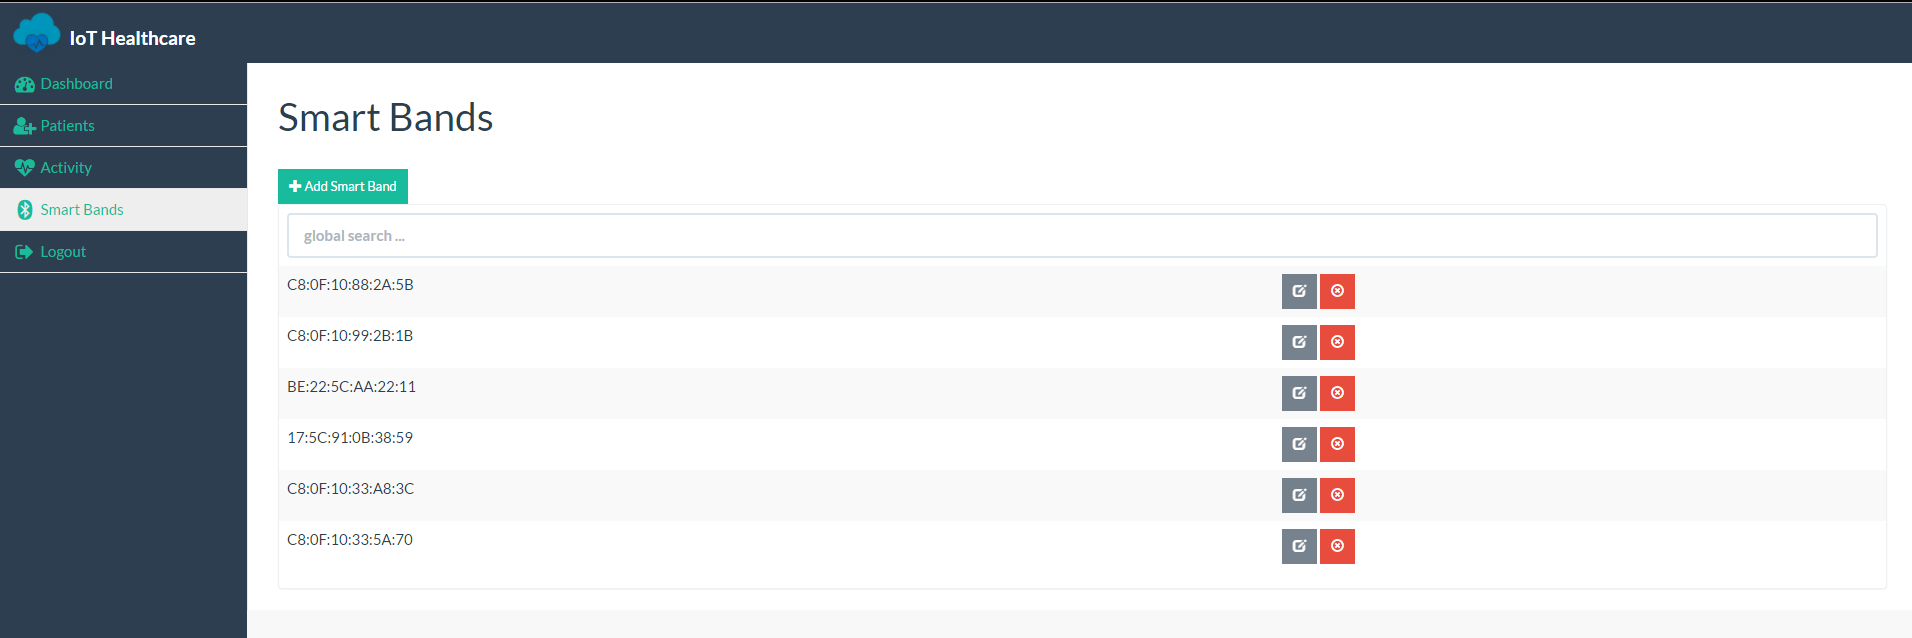
\includegraphics[width=1\textwidth]{./images/iothsmartbands}
	\rule{1\textwidth}{1pt}
	\caption{IoT Healthcare smartbands page}
\end{figure}


\subsubsection*{Patients}
In the patients page you can manage all the patients, each patient can have linked a specific smart band.

\begin{figure}[h!]
	\centering
	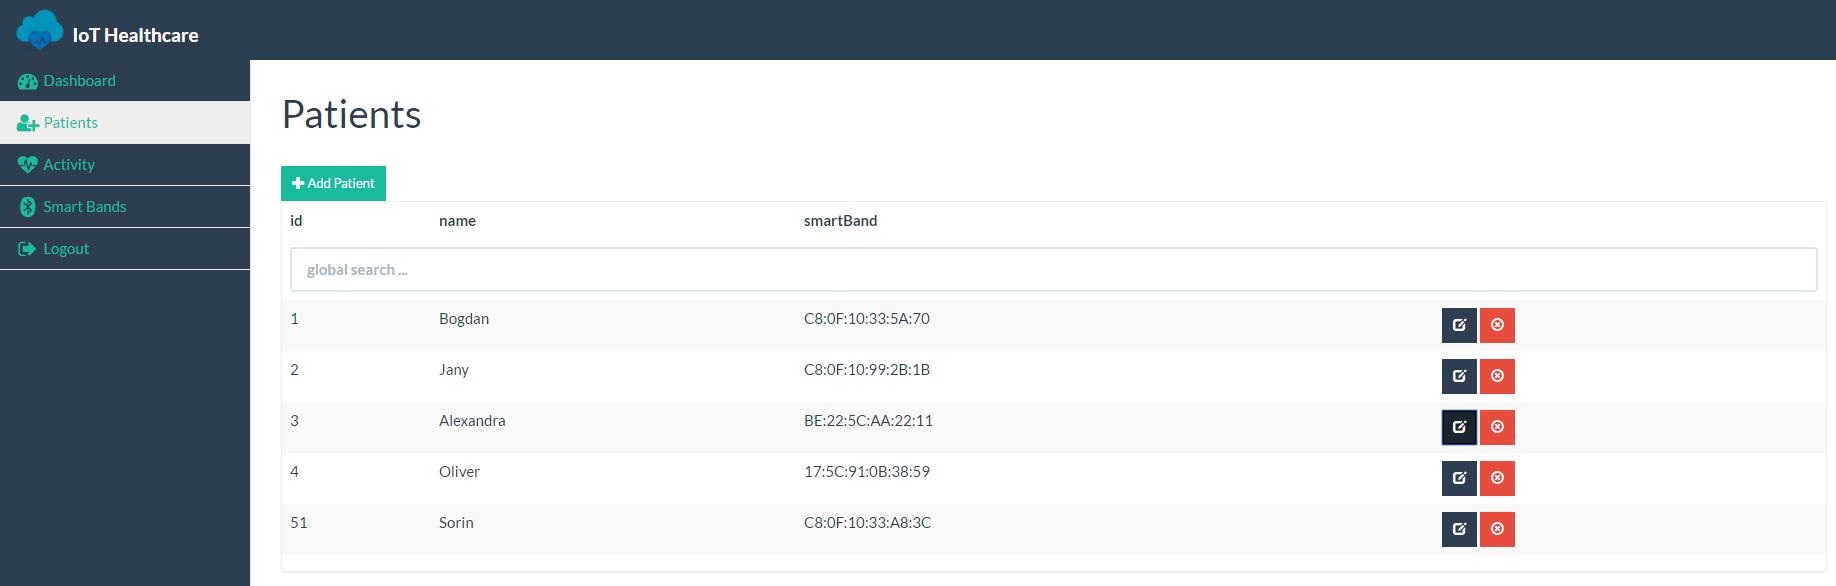
\includegraphics[width=1\textwidth]{./images/iothpatient}
	\rule{1\textwidth}{1pt}
	\caption{IoT Healthcare patients page}
\end{figure}

\subsubsection{Activity}
In the activity tab here is where the magic is happening. The daemon is sending an activity record every 20 min for each patient the record object has the number steps, an array of the heart rate values, the mac address of the smartband and of course the timestamp. 
\begin{lstlisting}[language=Bash] 
{
	"steps": 500,
	"heartRate": [
		43,
		89,
		30,
		40,
		0,
		5
	],
	"smartBand": {
		"mac": "C8:0F:10:88:2A:5B"
	},
	"timestamp": 1492617449907   
}
\end{lstlisting}      

\begin{figure}[h!]
	\centering
	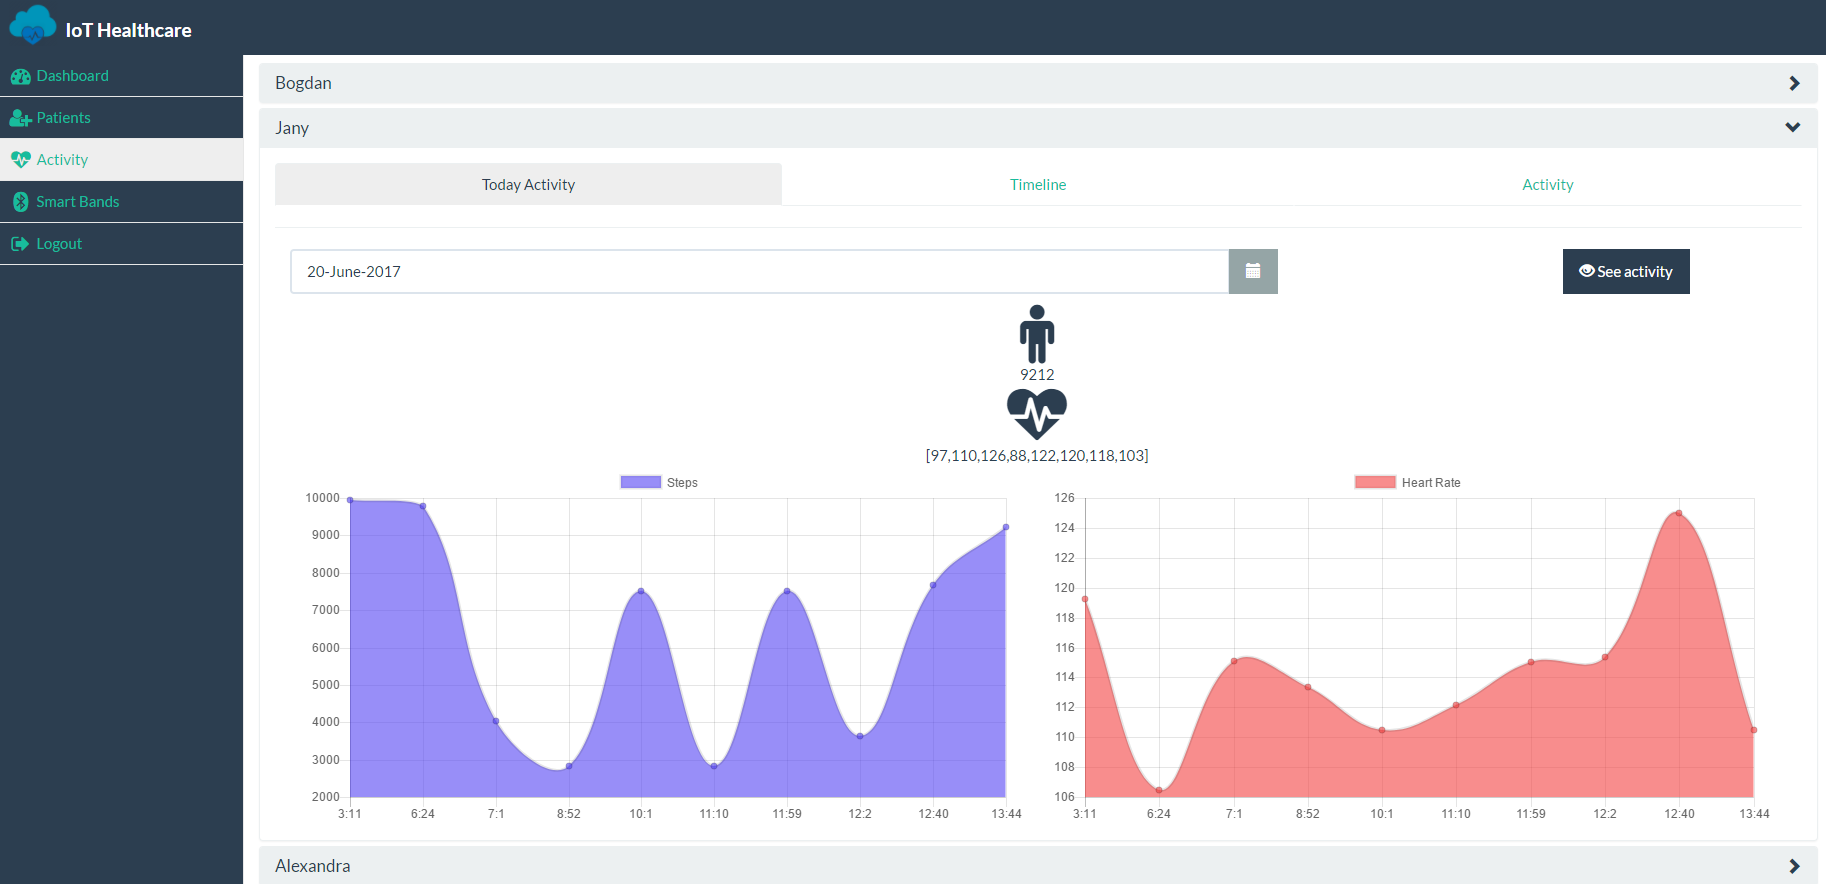
\includegraphics[width=1\textwidth]{./images/iothactivity}
	\rule{1\textwidth}{1pt}
	\caption{IoT Healthcare activity page}
\end{figure}

\section{Conclusions}

Lorem ipsum dolor sit amet, consectetur adipiscing elit. Duis in diam vel elit semper consequat. Quisque molestie ultricies erat, id porta elit tempus nec. Suspendisse eu diam nulla. Quisque sollicitudin semper eros eu vehicula. Suspendisse at vehicula odio, vitae fermentum libero. Mauris in sodales quam. Nullam facilisis finibus egestas. Duis id ipsum ut elit bibendum lobortis ut vel magna. Nullam at lacus sagittis, pharetra tortor quis, vestibulum mauris. Proin nec est erat. Vestibulum ante ipsum primis in faucibus orci luctus et ultrices posuere cubilia Curae; Aliquam erat volutpat. Donec ipsum tellus, sollicitudin vel nisi vel, convallis ultricies nulla. Praesent pellentesque ultrices sodales. Duis ante tellus, dapibus at euismod a, tempor eu massa.

Morbi rhoncus ligula id nibh luctus porttitor. Mauris ante purus, volutpat eget nisi eu, malesuada facilisis nisi. In ullamcorper condimentum scelerisque. Fusce eleifend mollis ex, iaculis consectetur lectus consectetur at. Donec id dignissim odio, non pretium sem. Curabitur gravida risus id interdum efficitur. Fusce dolor dui, condimentum in ullamcorper et, malesuada eget eros. Ut mollis lorem turpis, quis faucibus justo commodo et. Maecenas tellus massa, tempor at aliquam vel, rhoncus vulputate tortor.

Suspendisse sit amet eros in ligula feugiat interdum vel et ligula. Quisque pellentesque massa ut ipsum iaculis, quis porttitor ipsum accumsan. Morbi suscipit, enim et placerat laoreet, purus velit porttitor elit, auctor congue nunc arcu sit amet orci. Vestibulum dapibus, libero eu pulvinar porta, velit massa tincidunt metus, id imperdiet ipsum justo ut velit. Vivamus eget risus ante. Etiam elementum posuere erat ac accumsan. Pellentesque id hendrerit nulla. Mauris cursus risus ut cursus consectetur. Suspendisse venenatis quis ipsum a egestas.

Vestibulum placerat ex vitae ipsum efficitur pharetra. Aenean condimentum commodo libero, eu venenatis mauris ultrices bibendum. Nullam sit amet vehicula sapien, nec vulputate leo. Ut ipsum diam, rutrum ac rhoncus vel, pellentesque in metus. Vestibulum et metus at elit semper accumsan. Pellentesque finibus eros ante, vel ultricies risus accumsan sed. Donec pretium viverra eros quis vehicula.

Etiam et aliquet ex, non sagittis libero. Quisque non lorem efficitur, dapibus risus quis, maximus ipsum. Fusce eu mattis erat. Aliquam in sapien vitae ante bibendum ultrices. Sed vel lorem in arcu efficitur sagittis. Etiam tincidunt magna eu felis cursus, sed venenatis ex vulputate. Morbi semper rhoncus ultricies. Vivamus a aliquam risus, commodo fringilla nulla.